\documentclass{bioinfo}
\copyrightyear{2016}
\pubyear{2016}



%\usepackage{epsfig,multicol}
\usepackage{epsfig}
\usepackage{graphicx}
\usepackage{amsthm}
\usepackage{amssymb}
\usepackage{amsmath}
\usepackage{amsfonts}
\usepackage{mathrsfs}
\usepackage{multirow}
\usepackage{pbox}
%\usepackage{algorithm}
%\usepackage{algorithmic,subfigure}
\usepackage{url}

%\usepackage{vmargin}
%\setmarginsrb{1in}{1in}{1in}{1in}{0pt}{0pt}{0pt}{6mm}

\usepackage{color}
%\def\comm#1{\marginpar{\textcolor{red}{*\raggedright{\small #1}*}}}


%\documentclass{siamltex}



\newtheorem{proposition}{Proposition}
\newtheorem{lemma}{Lemma}
\newtheorem{theorem}{Theorem}
\newtheorem{corollary}{Corollary}
\newtheorem{definition}{Definition}

%\newtheorem{thm}{Theorem}

%\newtheorem{obs}{Observation}

\newtheorem{claim}{Claim}

\usepackage{multirow}

\newcommand{\Oh}[1]
	{\ensuremath{\mathcal{O}\!\left({#1}\right)}}
\newcommand{\access}
	{\ensuremath{\mathsf{access}}}
\newcommand{\rank}
	{\ensuremath{\mathsf{rank}}}
\newcommand{\select}
	{\ensuremath{\mathsf{select}}}
\newcommand{\occ}
	{\ensuremath{\mathsf{occ}}}
\newcommand{\nodelabel}
	{\ensuremath{\mathsf{label}}}
\newcommand{\BWT}
	{\ensuremath{\mathsf{BWT}}}
\newcommand{\C}
	{\ensuremath{\mathsf{C}}}
\newcommand{\LF}
	{\ensuremath{\mathsf{LF}}}
\newcommand{\Psiop}
	{\ensuremath{\mathsf{\Psi}}}
\newcommand{\mus}[1]
	{\SI{#1}{\micro\second}}
	
\newcommand{\elabel}{\ensuremath{\mathsf{label}}}
\newcommand{\EBWT}{\ensuremath{\mathsf{EBWT}}}


\def\ours{\mbox{\rm {\sc Vari}}}






\begin{document}
\firstpage{1}

\title[Succinct Colored de Bruijn Graphs]{Succinct Colored de Bruijn Graphs}

\author[Muggli, et al.]{Martin D. Muggli$^{1}$\footnote{to whom correspondence should be addressed} \footnote{The authors wish it to be known that, in their opinion, the first two authors should be regarded as joint First Authors.}, 
  Alexander Bowe$^{2}$\footnotemark[2],
  Noelle R. Noyes$^{3}$,
Paul Morley$^{3}$,
Keith Belk$^{4}$,
Robert Raymond$^{1}$,
Travis Gagie$^{5}$, 
Simon J. Puglisi$^{6}$,
Christina Boucher$^{1}$}

%% \author[Sample \textit{et~al}]{Corresponding Author\,$^{1,*}$, Co-Author\,$^{2}$ and Co-Author\,$^2$\footnote{to whom correspondence should be addressed}}
\address{$^{1}$Department of Computer Science, Colorado State University, Fort Collins, CO\\
  $^{2}$National Institute of Informatics, Chiyoda-ku, Tokyo, Japan\\
    $^{3}$Department of Clinical Sciences, Colorado State University, Fort Collins, CO\\
  $^{4}$Department of Animal Sciences, Colorado State University, Fort Collins, CO\\
  $^{5}$School of Computer Science and Telecommunications, Diego Portales University, Santiago, Chile\\
  $^{6}$Department of Computer Science, University of Helsinki, Finland}

\history{Received on XXXXX; revised on XXXXX; accepted on XXXXX}

\editor{Associate Editor: XXXXXXX}

\maketitle

\begin{abstract}
  



%\begin{abstract}

%In the 20 years since it was introduced to bioinformatics by Idury and Waterman, the {\em de Bruijn graph} has become a mainstay of modern genomics, essential to genome assembly.
%The wide use and importance of de Bruijn graphs has led to a number of succinct representations, which aim to implement the graph in small space, while still supporting fast navigation operations.
  \section{Motivation:}
%  \noindent
  Iqbal et al. (Nature Genetics, 2012) introduced the {\em colored de Bruijn graph}, a variant of the classic de Bruijn graph, which is aimed at ``detecting and genotyping simple and complex genetic variants in an individual or population''.
Because they are intended to be applied to massive population level data, it is essential that the graphs be represented efficiently.
Unfortunately, current succinct de Bruijn graph representations are not directly applicable to the colored de Bruijn graph, which requires additional information to be succinctly encoded as well as support for non-standard traversal operations.
\section{Results:}
Our data structure dramatically reduces the amount of memory required to store and use the colored de Bruijn graph, with some penalty to runtime, allowing it to be applied in much larger and more ambitious sequence projects than was previously possible.
\section{Availability:} https://github.com/cosmo-team/cosmo/tree/VARI
%\end{abstract}

  

\section{Contact:} \href{martin.muggli@colostate.edu}{martin.muggli@colostate.edu}
\end{abstract}

\section{Introduction}\label{sec:introduction}

\section{Introduction}

In the 20 years since it was introduced to bioinformatics by ~\cite{IW95}, the {\em de Bruijn graph} has become a mainstay of modern genomics, essential to genome assembly~\citep{Compeau11,sequel,ismb2015}. The near ubiquity of de Bruijn graphs has led to a number of succinct representations, which aim to implement the graph in small space, while still supporting fast navigation operations.  Formally, a de Bruijn graph constructed for a set of strings (e.g., sequence reads) has a distinct vertex $v$ for every unique $(k - 1)$-mer (substring of length $k - 1$) present in the strings, and a directed edge $(u, v)$ for every observed $k$-mer in the strings with $(k - 1)$-mer prefix $u$ and $(k - 1)$-mer suffix $v$. A contig corresponds to a non-branching path through this graph. See~\citep{Compeau11} for a more thorough explanation of de Bruijn graphs and their use in assembly. 

\cite{ICTFM12} introduced the {\em colored de Bruijn graph}, a variant of the classical structure, which is aimed at ``detecting and genotyping simple and complex genetic variants in an individual or population.'' The edge structure of the colored de Bruijn graph is the same as the classic structure, but now to each vertex ($(k - 1)$-mer) and edge ($k$-mer)
% FIXME: node coloring (CORTEX) looses information preserved in edge coloring(VARI), should we discuss this?  i.e. two nodes with the same color may or may not have a connecting edge with that color, but if you only color the nodes, you can't tell which is the case
is associated a list of colors corresponding to the samples in which the vertex or edge label exists. More specifically, given a set of $n$ samples, there exists a set $\mathcal{C}$ of $n$ colors $c_1, c_2, .., c_n$ where $c_i$ corresponds to sample $i$ and all $k$-mers and $(k-1)$-mers that are contained in sample $i$ are colored with $c_i$. A {\em bubble} in this graph corresponds to an undirected cycle, and is shown to be indicative of biological variation by \cite{ICTFM12}. 
{\sc Cortex}, the implementation of \cite{ICTFM12}, uses the colored de Bruijn graph to develop a method of assembling multiple genomes simultaneously, without losing track of the individuals from which $(k - 1)$-mers (and $k$-mers) originated. This graph is derived from either multiple reference genomes, multiple samples, or a combination of both.

Variant information of an individual or population can be deduced from structure present in the colored de Bruijn graph and the colors of each $k$-mer.
As implied by \cite{ICTFM12}, the ultimate intended use of colored de Bruijn graphs is to apply it to massive, population-level sequence data that is now abundant due to next generation sequencing technology (NGS) and multiplexing. These technologies have enabled production of sequence data for large populations, which has led to ambitious sequencing initiatives that aim to study genetic variation for agriculturally and bio-medically important species.  These initiatives include the {\em Genome 10K} project that aims to sequence the genomes of 10,000 vertebrate species~\citep{Haussler:2009}, the {\em iK5} project~\citep{Robinson:2011}, the 150 Tomato Genome ReSequencing project~\citep{tomato1,tomato2}, and the 1001 Arabidopsis project, a worldwide initiative to sequence cultivars of {\em Arabidopsis}~\citep{arabidopsis}.  Hence, the succinct colored de Bruijn graph is applicable in the context of these projects, in that it can assist in variation discovery within a species by analyzing all the data in these projects at once. 

In addition to species-specific initiatives, scientific and regulatory agencies are showing increased interest in shotgun metagenomic sequences for public health purposes~\citep{EMBL-EBI-Metagenomics,Miller2013}, specifically monitoring for antimicrobial resistance (AMR)~\cite{baquero_metagenomic_epi, port_2014_metagenomics_AMR_monitoring}.  AMR is considered one of the top public health threats, with fears that the spread of AMR will lead to increased morbitiy and mortality for many bacterial illnesses~\citep{CARB,FAOActionPlan2016}.  AMR occurs when bacteria express genetic elements that render them impervious to antibiotic treatments.  Importantly, these genetic resistance elements can be exchanged between distantly-related bacteria via multiple genetic mechanisms, which makes AMR an inherently population-level phenomenon~\citep{Baquero2013}.   Shotgun metagenomic sequencing allows access to the entire microbial population in a sample (the "metagenome"), which is of immense value for tracking and understanding the evolution of resistance elements within and across diverse bacteria\citep{MacLean2010}.  This metagenomics approach to AMR surveillance has been applied in both human and agricultural settings~\citep{noyes2016resistome,King2016}, generating hundreds of samples with terabytes of sequence data for relatively small studies.  Given the large number of samples and large size of sequence data involved in these whole-genome and metagenomic projects, it is imperative that the colored de Bruijn graph can be stored and traversed in a space- and time-efficient manner.
 
%the {\em Genome 10K} project that aims to sequence the genomes of 10,000 vertebrate species \cite{Haussler:2009}, the {\em iK5} project where the objective is to sequence the genomes of 5,000 arthropods \cite{Robinson:2011}, the 150 Tomato Genome ReSequencing project that aims to identify the sequence diversity within tomato \cite{tomato}, and the 1001 Arabidopsis  Project that is a worldwide initiative to sequence cultivars of Arabidopsis \cite{arabidopsis}. Given the large number of individuals and sequence data involved in these projects it is imperative that the colored de Bruijn graph is able to be stored and traversed in both a memory and time efficient manner.

\paragraph{Our Contribution}  
We develop an efficient data structure for storage and use of the colored de Bruijn graph. Compared to {\sc Cortex}, the implementation of \cite{ICTFM12}, our new data structure dramatically reduces the amount of memory required to store and use the colored de Bruijn graph, with some penalty to runtime. We demonstrate this reduction in memory through a comprehensive set of experiments across the following three datasets: (1)  four plant genomes, (2) 3,765 {\em Escherichia coli} assemblies,
 and (3) 87 sequenced metagenomic samples from commercial beef production facilities.  We show our method, which we refer to as $\ours$ (Finnish for color), has better peak memory usage on all these datasets. Our plant reference genomes dataset required 101 GB of RAM for  {\sc Cortex} to represent while $\ours$ required only 4 GB.  And  our
largest two datasets contain too many $k$-mers and colors for {\sc Cortex}'s data structure to represent in the 512 GB of RAM available on our bioinformatics servers. $\ours$ is a novel generalization of the succinct data structure for classical de Bruijn graphs due to \cite{BOSS12}, which is based on the Burrows-Wheeler transform of the sequence reads, and thus, has independent theoretical importance.

In addition to demonstrating the memory and runtime of $\ours$, we validate its output using the {\em E.coli} reference genome and a simulated variant.
%s 


\paragraph{Related Work} As noted above, maintenance and navigation of the de Bruijn graph is a space and time bottleneck in genome assembly. Space-efficient representations of de Bruijn graphs have thus been heavily researched in recent years. One of the first approaches was introduced by \cite{Simpson:2009} as part of the development of the ABySS assembler.  Their method stores the graph as a distributed hash table and thus requires 336 GB to store the graph corresponding to a set of reads from a human genome ($>$38x depth paired-end reads from Illumina Genome Analyzer II, HapMap: NA18507\footnote{\url{https://www.ncbi.nlm.nih.gov/sra/?term=SRA010896}}). 
 
 \cite{conway} reduced space requirements by using a sparse bitvector  (by \cite{bitvector}) to represent the $k$-mers (the edges), and used rank and select operations (to be described later) to traverse it. As a result, their representation took 32 GB for the same data set.  Minia, by \cite{wabi}, uses a Bloom filter to store edges. They traverse the graph by generating all possible outgoing edges at each node and testing their membership in the Bloom filter. Using this approach, the graph was reduced to 5.7 GB on the same dataset.  Contemporaneously, \cite{BOSS12} developed a different succinct data structure based on the Burrows-Wheeler transform~\citep{BW94} that requires 2.5 GB.  The data structure of \cite{BOSS12} is combined with ideas from IDBA-UD~\citep{idbaud} in a metagenomics assembler called MEGAHIT~\citep{megahit}.  In practice MEGAHIT requires more memory than competing methods  but produces significantly better assemblies.   \cite{paul} implemented the de Bruijn graph using an FM-index and {\em minimizers}.   Their method uses 1.5 GB on the same NA18507 data.  \cite{BFT} released the Bloom Filter Trie, which is another succinct data structure for the colored de Bruiin graph; however, we were unable to compare our method against it since  it only supports the building and loading of a colored de Bruijn graph and does not contain operations to support our experiments.  SplitMEM~\citep{splitmem} is a related algorithm to create a colored de Bruijn graph from a set of suffix trees representing the other genomes. Lastly, Lin et al. \citep{Lin} point out the similarity between the breakpoint graph, which is traditionally viewed as a data structure to detect breakpoints between genome rearrangements, and the colored de Bruijn graph. 
 

\paragraph{Roadmap} In the next section, we describe our succinct colored de Bruijn graph data structure, generalizing the stucture for classic de Bruijn graphs presented by ~\cite{BOSS12}. Section~\ref{sec:results} then elucidates the practical performance of the new data structure, comparing it to {\sc Cortex}. Section~\ref{sec:conclusion} offers some concluding remarks.



%\section{Approach}

\begin{methods}
  \section{Methods}
  \section{Methods}
\label{sec:methods}

Our data structure for colored de Bruijn graphs is based on the succinct representation of individual de Bruijn graphs introduced by \cite{BOSS12}---which we refer to as the BOSS representation from the authors' initials---so we start by describing that representation.  We note that BOSS is itself a generalization of FM-indexes~\citep{FM05} obtained by extending the Burrows-Wheeler transform (BWT) from strings to the multisets of edge-labels of de Bruijn graphs.  We then give a general explanation of how we add colors, and finally give details of our implementation.

\subsection{BOSS Representation}
\label{subsec:boss}

Consider the de Bruijn graph \(G = (V, E)\) for a set of $k$-mers, with each $k$-mer \(a_0 \cdots a_{k - 1}\) representing a directed edge from the node labelled \(a_0 \cdots a_{k - 2}\) to the node labelled \(a_1 \cdots a_{k - 1}\), with the edge itself labelled \(a_{k - 1}\).  Define the nodes' co-lexicographic order to be the lexicographic order of their reversed labels.  Let $F$ be the list of $G$'s edges sorted co-lexicographically by their ending nodes, with ties broken co-lexicographically by their starting nodes (or, equivalently, by their $k$-mers' first characters).  Let $L$ be the list of $G$'s edges sorted co-lexicographically by their starting nodes, with ties broken co-lexicographically by their ending nodes (or, equivalently, by their own labels).  If two edges $e$ and $e'$ have the same label, then they have the same relative order in both lists; otherwise, their relative order in $F$ is the same as their labels' lexicographic order.  Defining the edge-BWT (EBWT) of $G$ to be the sequence of edge labels sorted according to the edges' order in $L$, so \(\elabel (L [h]) = \EBWT (G) [h]\) for all $h$, this means that if $e$ is in position $p$ in $L$, then in $F$ it is in position
\begin{equation*}
|\{d\,:\,d \in E,\ \elabel (d) \prec \elabel (e)\}| + \EBWT (G).\rank_{\elabel (e)} (p) - 1\,,
\end{equation*}
where \(\EBWT (G).\rank_{\elabel (e)} (p)\) is the number of times $\elabel (e)$ appears in \(\EBWT (G) [1,p]\).  It follows that if we have, first, an array storing \(|\{d\,:\,d \in E,\ \elabel (d) \prec c\}|\) for each character $c$ and, second, a fast rank data structure on \(\EBWT (G)\) then, given an edge's position in $L$, we can quickly compute its position in $F$.

Let $B_F$ be the bitvector with a 1 marking the position in $F$ of the last incoming edge of each node, and let $B_L$ be the bitvector with a 1 marking the position in $L$ of the last outgoing edge of each node.  Given a character $c$ and the co-lexicographic rank of a node $v$, we can use $B_L$ to find the interval in $L$ containing $v$'s outgoing edges, then we can search in \(\EBWT (G)\) to find the position of the one $e$ labelled $c$.  We can then find $e$'s position in $F$, as described above.  Finally, we can use $B_F$ to find the co-lexicographic rank of $e$'s ending node.  With the appropriate implementations of the data structures, we can store $G$ in \((1 + o (1)) |E| (\lg \sigma + 2)\) bits, where $\sigma$ is the size of the alphabet (i.e., 4 for DNA), such that when given a character $c$ and the co-lexicographic rank of a node $v$, in $\Oh{\log \log \sigma}$ time we can find the node reached from $v$ by following the directed edge labelled $c$, if such an edge exists.

If we know the range \(L [i..j]\) of $k$-mers whose starting nodes end with a pattern $P$ of length less than \((k - 1)\), then we can compute the range \(F [i'..j']\) of $k$-mers whose ending nodes end with \(P c\), for any character $c$, since
\begin{eqnarray*}
    i' & = & |\{d\,:\,d \in E,\ \elabel (d) \prec c\}| + \EBWT (G).\rank_c (i - 1)\\ 
    j' & = & |\{d\,:\,d \in E,\ \elabel (d) \prec c\}| + \EBWT (G).\rank_c (j) - 1\,.
\end{eqnarray*}
It follows that, given a node $v$'s label, we can find the interval in $L$ containing $v$'s outgoing edges in $\Oh{k \log \log \sigma}$ time, provided there is a directed path to $v$ (not necessarily simple) of length at least \(k - 1\).  In general there is no way, however, to use \(\EBWT (G)\), $B_F$ and $B_L$ alone to recover the labels of nodes with no incoming edges.

To prevent information being lost and to be able to support searching for any node given its label, Bowe et al.\ add extra nodes and edges to the graph, such that there is a directed path of length at least \(k - 1\) to each original node.  Each new node's label is a \((k - 1)\)-mer that is prefixed by one or more copies of a special symbol $\$$ not in the alphabet and lexicographically strictly less than all others.  Notice that, when new nodes are added, the node labelled $\$^{k - 1}$ is always first in co-lexicographic order and has no incoming edges.  Bowe et al.\ also attach an extra outgoing edge labelled $\$$, that leads nowhere, to each node with no original outgoing edge.  The edge-BWT and bitvectors for this augmented graph are, together, the BOSS representation of $G$.

\subsection{Adding Color}
\label{subsec:color}

We cannot represent the colored de Bruijn graph for a multiset \(\mathcal{G} = \{G_1, \ldots, G_t\}\) of individual de Bruijn graphs satisfactorily by simply representing each individual graph separately, for two reasons: first, the memory requirements would quickly become impractical and, second, we should be able to answer efficiently queries such as ``which individual graphs contain this edge?''  Therefore, we set $G$ to be the union of the individual graphs and build the BOSS representation only for $G$.  As long as most of the $k$-mers are common to most of the individual graphs, the memory needed to store $G$ is comparable to that need to store an individual graph.

To indicate which edges of $G$ are in which individual graphs, we build and store a two-dimensional binary array $C$ in which \(C [i, j]\) indicates whether the $i$th edge in $G$ is present in the $j$th individual de Bruijn graph (i.e., whether that edge has the $j$th color). 
(Recall from the description above of BOSS that we consider the edges in $G$ to be sorted lexicographically by the reversed labels of their starting nodes, with ties broken lexicographically by their own single-character labels.) 
If the individual graphs are sufficiently similar, then we can compress $C$ effectively and store it in such a way that we can still access its individual bits quickly and support fast rank and select queries on the rows.  (A $\select$ query on the $i$th row takes an argument $r$ and returns the index $j$ of the $r$th individual graph that contains the $i$th edge in $G$.)  In the next subsection we give details of some relatively simple compression strategies that support fast access, rank and select.  With these data structures, we can navigate efficiently in any of the individual graphs and switch between them.  For example, we can efficiently check whether an edge has a particular color (with an access), count the number of colors it has (with a $\rank$ query) or list them (with repeated $\select$ queries).  We have not yet considered more sophisticated compression schemes that could still offer fast queries while taking advantage of, e.g., correlations among the variations or grouping of the individual graphs by subpopulation.

Figure~\ref{fig:purple} shows an example of how we represent a colored de Bruijn graph consisting of two individual de Bruijn graphs.  Suppose we are at node {\tt ACG} in the graph, which is the co-lexicographically eighth node.  Since the eighth 1 in $B_L$ is \(B_L [10]\) and it is preceded by two 0s, we see that {\tt ACG}'s outgoing edges' labels are in \(\EBWT [8..10]\), so they are {\tt A}, {\tt C} and {\tt T}.  Suppose we want to follow the outgoing edge $e$ labelled {\tt C}.  We see from \(C [9, 0..1]\) (i.e., the tenth column in $C^\mathrm{T}$) that $e$ appears in the second individual graph but not the first one (i.e., it is blue but not red).    There are four edges labelled {\tt A} in the graph and three {\tt C}s in \(\EBWT (G) [0..9]\), so $e$ is \(F [6]\).  (Since edges labelled {\tt \$} have only one end, they are not included in $L$ or $F$.)  From counting the 1s in \(B_F [0..6]\), we see that $e$ arrives at the fifth node in co-lexicographic order that has incoming edges.  Since the first node, {\tt \$\$\$}, has no incoming edges, that means $e$ arrives at the sixth node in co-lexicographic order, {\tt CGC}.

\begin{figure*}
\footnotesize
\begin{tabular}{@{}c@{\hspace{0.03\textwidth}}c@{\hspace{0.03\textwidth}}c@{}}
\includegraphics[width=.31\textwidth]{purplegraph} &
\includegraphics[width=.31\textwidth]{newpurplemapping} &
\raisebox{11ex}{$\begin{array}{@{}rr@{}}
   \EBWT (G) = & \mathtt{TCCGTGGGACTAAA\$C}\\[1ex]
         B_F = & \mathtt{ 001111110111111}\\
         B_L = & \mathtt{1110111100111111}\\[1ex]
C^\mathrm{T} = & \mathtt{0000001001010000}\\
               & \mathtt{0000000110101001}
\end{array}$}
\end{tabular}
\caption{{\bf Left:} A colored de Bruijn graph consisting of two individual graphs, whose edges are shown in red and blue.  (We can consider all nodes to be present in both graphs, so they are shown in purple.)  {\bf Center:} The nodes sorted into co-lexicographic order, with each node's number of incoming edges shown on its left and the labels of its outgoing edges shown on its right.  The edge labels are shown in red or blue if the edges occur only in the respective graph, or purple if they occur in both.  {\bf Right:} Our representation of the colored de Bruijn graph: the edge-BWT and bitvectors for the BOSS representation for the union of the individual graphs, and the binary array $C$ (shown transposed) whose bits indicate which edges are present in which individual graphs.}
\label{fig:purple}
\end{figure*}

\subsection{Implementation}
\label{subsec:implementation}

We now give some details of how our data structure is implemented and constructed in practice.

\subsubsection{Data Structure}

The arsenal of component tools available to succinct data structures designers has grown considerably in recent years~\citep{Navarro16}, with many methods now implemented in libraries. We chose to make heavy use of the succinct data structures library (SDSL)\footnote{\url{https://github.com/simongog/sdsl-lite}} 
in our implementation.

\(\EBWT (G)\), the sequence of edge labels, is encoded in a wavelet tree, which allows us to perform fast rank queries, essential to all our graph navigations. The bitvectors of the wavelet tree  and the $B$ bitvector are stored in the Raman-Raman-Rao (RRR) encoding~\citep{RRR07}.
%[SJP: RRR will be significantly slower than a plain encoding, and I'm not sure it will reduce the size of the WT very much - this is something we need to test. We might even want to use something other than a WT].
The rows of the color matrix, $C$, are concatenated (i.e. $C$ is stored in row-major order) and this single long bit string is then compressed.  It is either stored with RRR encoding,  or alternately Elias-Fano encoding~\citep{elias1974efficient,fano1971number,bitvector} which supports online construction.  Online construction is important for datasets where $C$ is too large to fit in memory in uncompressed form, such as our metagenomic sample dataset.  These encodings reduce the size of $C$ considerably because we expect rows to be very sparse
%(i.e. most $k$-mers are contained in most samples),
and both encodings exploit this sparseness. 
%[SJP: we really should be using the access-optimised encoding that Travis and I suggested --- RRR is overkill and likely slower].

\subsubsection{Construction}


In order to convert the input data to the format required by BOSS (that is, in correct sorted order, including dummy edges and bit vectors), we use the following process.  We take care to ensure only subsets of data are needed in RAM at any one time during construction.

%First, 
%we read the header of the Cortex graph format, then iterate over the $(k-1)$-mers. For each $(k-1)$-mer, Cortex provides a bit matrix, where each row is a colour, and each
%column is a flag to indicate outgoing edges present in that colour. We invert this matrix to give us a bitmap representing the colours that each outgoing edge symbol is a member of.

Our construction algorithm takes as input the set of ($k$-mer, color-set) pairs present in the input sets of reads, or alternately, $k$-mer counts for each color which we convert to the former ourselves.
Here, color-set is a bit set indicating which samples the $k$-mer occurs in.
We provide the option to use the {\sc Cortex} frontend to generate the ($k$-mer, color-set). Unfortunately, this also limits the datasets to those that would run through {\sc Cortex}.  To overcome this, we provide the option to use a list of KMC2~\citep{KMC2} sorted $k$-mer counts as input.  With this option, the $k$-mers from each $k$-mer count file in native KMC2 binary format are streamed through a priority queue to produce the union of all $k$-mer sets; initially one $k$-mer from each file is tagged with  which file it originated from, and the ($k$-mer, file ID) pair is added to the queue.   The priority queue ensures the lexicographically smallest $k$-mer instances across all files can be popped off the queue consecutively.  All of the $k$-mer count files contributing a particular $k$-mer value have their corresponding color recorded as `1' bits in the bit set for that $k$-mer.  Both the $k$-mer and the bit set are then appended to vectors which optionally are allocated in external memory using the STXXL\footnote{\url{http://stxxl.sourceforge.net/}} library.   As each $k$-mer is popped off the queue, another $k$-mer is added to the queue to take the old $k$-mer's place (i.e. using the file identified by the popped $k$-mer's tag).  This process continues until all files are read in their entirety.  By both streaming data from the source files and streaming it to the external vectors, only a small amount of the data need exist in memory at a time; the priority queue will only contain the number of samples and only one row of the color matrix needs to exist in memory before being written out to disk.

%This effectively gives us ($k$-mer, color-set) pairs\footnote{In our current implementation, the color-set bitmaps were chosen to be 64 bits wide for simplicity, but can easily be extended to wider
%(or variable-length) bitmaps.}.

After constructing the initial union set of $k$-mers and their corresponding color rows, BOSS construction mostly continues as originally described by Bowe {\it et al.}.  The changes from the original construction algorithm are that most of the data optionally resides in external memory and the rows of the color matrix are permuted with their corresponding $k$-mers as they are sorted.  For each of the $k$-mers we generate the reverse complement (giving it the same color-set as its twin). Then, for each $k$-mer (including the reverse complements),
we sort the ($k$-mer, color-set) pairs by the first $k-1$ symbols (the source node of the edge) to give the $F$ table (from here, the colors are moved around with rows of $F$, but otherwise ignored until 
the final stage). Independently, we sort the $k$-mers (without the color-sets) by the last $k-1$ symbols (the destination node of the edge) to give the $L$ table.

With $F$ and $L$ tables computed, we calculate the set difference $F-L$ (comparing only the $(k-1)$-length prefixes and suffixes respectively), which tells us which nodes require incoming dummy edges. Each such node is then
shifted and prepended with $\$$ signs to create the required incoming dummy edges ($k-1$ each). These incoming dummy edges are then sorted by the first $k-1$ symbols.
Let this table of sorted dummy edges be $D$. Note that the set difference $L - F$ will give the nodes requiring outgoing dummy edges, but these do not require sorting, and so we can calculate it as is needed in the final stage.

Finally, we perform a three-way merge (by first $k-1$ symbols) $D$ with $F$, and $L-F$ (calculated on the fly). For each resulting edge, we keep track of runs of equal $k-1$ length prefixes,
and $k-2$ length suffixes of the source node, which allows us to calculate the $B_F$ and $B_L$ bit vectors, respectively. Next, we write the bit vectors, symbols from last column, and
count of the second to last column to a packed file on disk, and the colors to a separate file.   The color file is then either buffered in RAM and RRR encoded or optionally streamed from disk and then Elias-Fano encoded online (i.e. only the compressed version is ever resident).  The time bottleneck in the above process is clearly in sorting the $D$ and $F$ tables, which are of the same size, and are made up of elements of size $O(k)$. Thus, overall, construction of the data structure takes $O(k(|F|\log|F|))$ time.



%TODO: Asymptotics? We should also say that we use STXXL (which will give us EM sorting bounds)
% Reading: O(N) (# nodes) x O(sigma|C|)
% Sorting: O(|F| log |F|)
% F-L: O(|F|)
% Sort dummies: O(|D| log |D|)
% Final Merge: O(|F| + |D|) (|D| <= |F| -> O(|F|))

%[SJP: The following overly detailed description is from Alex. To be refined.]
%
%Getting + sorting necessary kmers
%1 read in the node, coverages and edge bitmaps
%2 iterate over the color bitmap, then in an inner loop iterate over
%edge symbols. I then make an inverted symbol by color bit matrix
%3 for each symbol that has a non-zerod row in the matrix, I shift the
%node and append the symbol to make a k-mer (edge)
%4 I reverse the nucleotides of the kmer so it will be sorted in colex
%order, and I also compute the reverse complement
%5 I add (kmer, color-bitmap), (revcomp, color-bitmap) pairs to a
%sorting container (which generates runs, then merges them on access
%later) which drops the last symbol before sorting (table F)
%6 I also add the kmer and revcomp (no color data) to another sorting
%container which sorts based on the whole string (table L)
%Note: In the old version, only 6 was done. The radix sort used two
%tables, so by saving the buffer table we had the second-last iteration
%as well, which meant we had table F
%Note: 5 and 6 are sorted in parallel on different disks for my
%version, so it is faster than a multi-pass version (tested), but also
%uses 2x the disk space. It isnt a radix sort though, so it doesnt
%double the table size. i.e. for both implementations, we use 2x the number 
%of input kmers to add rev comps, then 2x again for F and L.
%
%Generating incoming dummy edges:
%7. i use std::set-difference to take both tables (wrapping the
%iterator so access return just the first k-1 syms from kmers in of F,
%and the last k-1 syms from kmers in L, and both made to be unique - no
%duplicates). This calculates F - L, since any node without a
%predecessor needs an incoming dummy.
%8. it outputs the k-1-mers from F to a provided function, which loops
%(k-2) times to generate \$... \$\$... \$\$\$... (these extra shifts aren't
%technically needed, except to be able to generate the labels for
%incoming dummies again)
%9. each of these is added to another sorter, like above, to be sorted
%on their first k-1 symbols (with \$ sorting before any other symbols).
%Note: before 9, even without all the shifts, the dummies are output in
%the same order as L (colex of whole edge).
%Note: colors dont need to be looked at here (we treat dummies as
%having 0 color for now)
%
%Merging and outgoing dummies:
%Note: You could do a L-F set difference to get outgoing dummies, but
%they are generated in the right order for F, so I combined them into
%one big merge step at the end.
%10. I make a wrapped iterator to access F without the color
%information, but to save it to a color variable that is in scope. This
%way I can merge the color in as I'm writing the kmers out.
%11. I take the two tables F and L, and the dummies. I merge the
%dummies into F (although this time comparing all k symbols), but I
%also calculate the L-F set difference as I'm going. Kind of like a
%3-way merge. If a node is in L that isnt in F, I shift that node and
%append a $ on the right: ....$
%12. each of these is sent to a function, which checks all the first
%k-1 symbols, and last k-1 symbols to generate the B and B' vectors
%(which show the range of entries for nodes in L and F)
%13. the last symbol is written to a file along with the bit vectors
%(interleaved and packed into 64bit blocks)
%14. the color (which is a variable that is now overwritten by the
%iterator wrapper) is written to a separate file.
%
%
%\begin{figure}
%\begin{center}
%\includegraphics[width=.5\textwidth]{New+Doc+5_1.jpg} \\[10ex]
%\caption{Construction of the succinct colored de Bruijn graph, from input to output.}
%\label{fig:construction}
%\end{center}
%\end{figure}

\subsubsection{Traversal}
We implemented two traversal methods based on those of {\sc Cortex} with a modification in light of our intention to apply $\ours$ to metagenomic reads looking for AMR gene presence.

The first, {\it bubble calling}, is a simple algorithm to detect sequence variation in genomic data. It consists of iterating over a set of $k$-mers in order to find places where bubbles start and terminate.  When combined with the $k$-mer color (in a colored de Bruijn graph), this enables identification of places where genomic sequences diverge from one another.  The differing region of the two sequences will form the two arms of a bubble, each colored with only one of the two sequence's colors.  A bubble is identified when a vertex has two outgoing edges. Each edge is followed in turn to navigate a non-branching path until reaching a vertex with two incoming edges. If the terminating vertex is the same for both paths, we call this a bubble. Colors for the bubbles are determined by looking at the color assignment of the corresponding $(k)$-mers. Our implementation in $\ours$ closely follows the pseudocode given by \cite{ICTFM12}.
%; however, it navigates the graph only in a forward direction to see if both paths converge at the same vertex, while {\sc Cortex} navigates the graph backwards and forwards to find a path of adjacent vertices.


{\sc Cortex}'s traversal algorithms were designed for single isolates. For the beef safety experiments, which use metagenomic samples, we implemented a traversal inspired by {\sc Cortex}'s {\it path divergence} algorithm.  In the original {\sc Cortex} path divergence algorithm, bubbles are identified where a user-supplied reference sequence prescribes a walk through a (possibly tangled) sections of the graph in one arm of a bubble while the alternative arm must be branch free.  This branch free requirement on the second arm could be a problem for metagenomic data. Due to the presence of tangle inducing homologous genomes and risk of inferring erroneous, chimeric sequences (which comprise reads from a mix of genomes in the sample), variant detection in metagenomic data is more complex. % FIXME: citation required?
In the absence of a simple metagenomic-aware traversal algorithm, we implemented a variation of the path divergence algorithm which addresses a simpler problem, primarily for the purpose of measuring performance.  This algorithm uses a reference guided approach and allows us to measure the memory footprint at traversal time as well as the time savings of not traversing the entire dataset.  For this purpose, we focus specifically on the presence of AMR genes (our reference sequence) rather than variants of those genes; in our derived algorithm we ignore sample path segments leading away from and returning to the AMR gene path.  This avoids some of the problems with tangles, incomplete coverage, or read errors.  Thus as we traverse the gene path, we simply count the number of samples in each sample group that color the current edge.   We note that keeping $C$ in row major order allows us to compute this count in constant time as the difference between two $\rank$ queries.  







%% \subsubsection{{\sc\bf Cortex}'s Graph Implementation}

%% Before discussing our experimental results, we give a brief description of the colored de Bruijn graph data structure that is implemented in the current {\sc Cortex} release, which we use as a baseline to measure our performance against in the next section. 

%% {\sc Cortex} implements the colored de Bruijn graph using a hash table. Each entry in the hash table stores a $(k - 1)$-mer (vertex in the graph) as well as the following fields: the $(k-1)$-mer labelling this vertex, {\sf coverage} (an array, indexed by color), {\sf status}, and {\sf edges} (indicating adjacent $(k - 1)$-mers in the graph). 

%% The $(k-1)$-mer part of the hashtable entry is a compile time determined length, composed of multiple 64-bit fields (sufficient to accommodate $k-1$ nucleotides, represented as two bits each).
%% The coverage information is used for error correction prior to graph construction, e.g., to remove low-coverage $k$-mers assumed to be the result of sequence errors. Later, when processing the graph, the {\sf coverage} array is used to determine if a $k$-mer exists for a given color (coverage of 0 for a given color indicates the $(k-1)$-mer does not exist in that sample). The {\sf status} field is used at runtime to record whether the vertex has been previously visited, and to store other information specific to a given algorithm (e.g. bubble finding). Finally, an {\sf edges} field is stored for each $k$-mer and each color. It is one byte in size, and each of the eight bits indicate which bases precede and follow the $k$-mer for this color. Since there are four possible predecessors and successors, one byte is sufficient.

\end{methods}

%\section{Results}

In this section, we present our experimental results on {\em E. coli} and GenomeTrakr data. We show the scalability of $\ours$ by demonstrating the time and computational resources needed to build the colored de Bruijn graph for 16,000 strains of salmonella.  Next, in order to validate the correctness of our approach, we generated two succinct colored de Bruijn graphs with sets of three  \emph{E. coli} assemblies each, merged them, and verified its equivalence to a six color graph built from scratch.  This experiment demonstrates that the merged colored de Bruijn graph is equivalent to that produced by building the graph without merging.    We ran all performance experiments on a machine with two Xeon E5-2640 v4 chips, each having 10 2.4 GHz cores.  The system contains 755 GB of RAM and two ZFS RAID pools of 9 disk each for storage.  We report wall clock time and maximum resident set size from Linux.  We use the SDSL-Lite library~\cite{SDSL} to store all succinct vectors. %We report all time in CPU time.
 

%%%%%%%%%%%%%%%%%%%%%%%%%%%%%%%%%%%%%%%%%%%%%%%%%%%%%%%%%%%%%%%%%%%%%%%%%%%%%%%%%%%%%%%%%%%%%%%%%%%%%%%%%%%%%%%%%%%%%%%%%%%%%%%%%

\begin{table*}[t]
\footnotesize
\begin{center}
%\vspace{8mm}
%{\setlength{\tabcolsep}{1em}
\begin{tabular}{|l|r|r|r|r|r|r|r|r|r|r|r|r|}
  \hline
  &  \multicolumn{2}{|c|}{Input Stats} & \multicolumn{3}{|c|}{de Bruijn Graph } & \multicolumn{3}{|c|}{Color Matrix } & \multicolumn{4}{|c|}{Combined Requirements}\\
  \hline

\textbf{Program and Dataset} & \textbf{$k$-mers} & \textbf{Colors} & \textbf{ RAM}& \textbf{Time} & \textbf{Size} & \textbf{RAM} &   \textbf{Time} & \textbf{Size} &  \textbf{RAM}  & \textbf{Ext. Mem.}  &   \textbf{Time} & \textbf{Size} \\ 
\hline

$\vari$(8k-1)   & 2.4 B       & 8,000 &              271 GB      & 30 h 49 m & 0.63 GB &              117 GB     & 6 h 28 m   & 114 GB              &    271 GB  & 4.6 TB  & 37 h  27 m &  114 GB \\
$\ours$(8k-1)      & 2.4 B     & 8,000 &              137 GB      & 21 h 27 m & 0.63 GB &              117 GB    & 5 h 3 m    & 114 GB               &    137 GB  & 1.5 TB  & 26 h  30 m & 114 GB\\


%$\vari$-C(8k-1) & 2.4 B    & 8,000 & 117 GB & N/A     & 6 h 28 m & 106 GB \\

\hline

\hline
\end{tabular}
\label{tab:compare}
\caption{Comparison between building a succinct colored de Bruijn for the same 8,000 Salmonella strains using $\vari$ versus $\ours$.}
%\caption{Performance statistics for $\vari$ and $\ours$. We separately list the succinct de Bruijn graph producing programs (labeled $\vari$ and $\ours$) from the color annotation matrix producing programs (labeled $\vari$-C and $\ours$-C). The total size of a succinct colored de Bruijn graph is comprised of the space for the succinct de Bruijn graph plus the space for the color matrix. }
\end{center}
\end{table*}
%%%%%%%%%%%%%%%%%%%%%%%%%%%%%%%%%%%%%%%%%%%%%%%%%%%%%%%%%%%%%%%%%%%%%%%%%%%%%%%%%%%%%%%%%%%%%%%%%%%%%%%%%%%%%%%%%%%%%%%%%%%%%%%%%

%%%%%%%%%%%%%%%%%%%%%%%%%%%%%%%%%%%%%%%%%%%%%%%%%%%%%%%%%%%%%%%%%%%%%%%%%%%%%%%%%%%%%%%%%%%%%%%%%%%%%%%%%%%%%%%%%%%%%%%%%%%%%%%%%
\begin{table*}[t]
\footnotesize
\begin{center}
%\vspace{8mm}
%{\setlength{\tabcolsep}{1em}
\begin{tabular}{|r|r|r|r|r|r|r|r|r|r|r|r|r|}
  \hline
  &  \multicolumn{2}{|c|}{Input Stats} & \multicolumn{3}{|c|}{de Bruijn Graph } & \multicolumn{3}{|c|}{Color Matrix } & \multicolumn{4}{|c|}{Combined Requirements}\\
  \hline

\textbf{Program and Dataset} & \textbf{$k$-mers} & \textbf{Colors} & \textbf{ RAM}& \textbf{Time} & \textbf{Size} & \textbf{RAM} &   \textbf{Time} & \textbf{Size} &  \textbf{RAM}  & \textbf{Ext. Mem.}  &   \textbf{Time} & \textbf{Size} \\ 
\hline
$\vari$(4k-1)      & 1.1 B    & 4,000 &               136 GB      & 8 h 46 m  & 0.31 GB &              52 GB     & 1 h 39 m & 51.2 GB               & 136 GB & 1 TB    & 10 h 25 m & 51 GB \\
$\vari$(4k-2)      & 1.5 B    & 4,000 &              137 GB      & 10 h 40 m & 0.52 GB &              54 GB     & 2 h 22 m & 52.5 GB                &  137 GB & 1.5 TB  &  13 h  2 m & 53 GB\\
$\merge$(4k-1, 4k-2)  & 2.4 B    & 8,000 &              10 GB       & 2 h 1 m   & 0.63 GB &              117 GB    & 1 h  2 m & 106 GB               &  117 GB    &  N/A    &  3 h 3 m & 106 GB \\

\hline
$\ours$(8k-1)      & 2.4      & 8,000 &              137 GB      & 21 h 27 m & 0.63 GB &              117 GB    & 5 h 3 m  & 117 GB               &    137 GB  & 1.5 TB  & 26 h  30 m & 106 GB\\

%$\vari$-C(4k-1) & 1.1 B    & 4,000 & 52 GB  & N/A     & 1 h 39 m & 51.2 GB \\
%$\vari$-C(4k-2) & 1.5 B    & 4,000 & 54 GB  & N/A     & 2 h 22 m & 52.5 GB \\
%$\ours$-C(4k-1, 4k-2)  & 2.4 B & 8,000 & 117 GB & N/A & 1 h 2 m & 106 GB \\
\hline



\hline
\end{tabular}
\label{tab:breakdown}
\caption{Breakdown of the components of $\ours$ which was listed in Table 1. The $\ours$ method consists of running $\vari$ on subsets of the population (4k-1 and 4k-2) and then merging the results with our proposed merge algorithm (denoted merge here).  Here we list the resources used for both individual runs of VARI as well as the merge.  We also list the combined resources, consisting of the total time and maximum space used across all three components of $\ours$ used in this dataset. Both $\vari$ and our merge algorithm each consist of two programs: one primarily responsible for the succinct de Bruijn graph and one for compressing the color matrix.  The resources for these are listed in separate columns and the combined resources needed for each method in the rightmost columns.  Size is the resulting succinct data structure size.}
%\caption{Performance statistics for $\vari$ and $\ours$. We separately list the succinct de Bruijn graph producing programs (labeled $\vari$ and $\ours$) from the color annotation matrix producing programs (labeled $\vari$-C and $\ours$-C). The total size of a succinct colored de Bruijn graph is comprised of the space for the succinct de Bruijn graph plus the space for the color matrix. }
\end{center}
\end{table*}
%%%%%%%%%%%%%%%%%%%%%%%%%%%%%%%%%%%%%%%%%%%%%%%%%%%%%%%%%%%%%%%%%%%%%%%%%%%%%%%%%%%%%%%%%%%%%%%%%%%%%%%%%%%%%%%%%%%%%%%%%%%%%%%%%



%%%%%%%%%%%%%%%%%%%%%%%%%%%%%%%%%%%%%%%%%%%%%%%%%%%%%%%%%%%%%%%%%%%%%%%%%%%%%%%%%%%%%%%%%%%%%%%%%%%%%%%%%%%%%%%%%%%%%%%%%%%%%%%%%
\begin{table*}[h!]
\footnotesize
\begin{center}
%\vspace{8mm}
%{\setlength{\tabcolsep}{1em}
\begin{tabular}{|l|r|r|r|r|r|r|r|r|r|r|r|r|}
  \hline
  &  \multicolumn{2}{|c|}{Input Stats} & \multicolumn{3}{|c|}{de Bruijn Graph} & \multicolumn{3}{|c|}{Color Matrix} & \multicolumn{4}{|c|}{Combined Requirements}\\
  \hline

\textbf{Program and Dataset} & \textbf{$k$-mers} & \textbf{Colors} & \textbf{ RAM}& \textbf{Time} & \textbf{Size} & \textbf{RAM} &   \textbf{Time} & \textbf{Size} &  \textbf{RAM}  & \textbf{Ext. Mem.}  &   \textbf{Time} & \textbf{Size} \\ 
\hline

%$\vari$(4k-1)      & 1.1 B    & 4,000 &               136 GB      & 8 h 46 m  & 0.31 GB &              52 GB     & 1 h 39 m & 51.2 GB               & 136 GB & 1 TB    & 10 h 25 m & 51 GB \\
$\vari$(4k-3)       & 1.7 B    &  4,000 &              135 GB      & 10 h 53 m & 0.46 GB &              53 GB     & 2 h 34 m & 51.8 GB               & 135 GB & 1.6 TB  & 13  h  27 m     & 52 GB \\
$\vari$(4k-4)       & 2.4 B    &  4,000 &              137 GB      & 14 h 35 m & 0.67 GB &              59 GB     & 3 h 37 m & 57.9 GB               & 137 GB & 2.34 TB & 18 h   12 m         & 59 GB\\

$\merge$(4k-3, 4k-4)   & 3.8 B    & 8,000  &              17 GB       & 2 h 59 m  & 1.00 GB &              118 GB    &  57 m    & 107 GB                &  118 GB & N/A     &     3 h 56 m             & 108 GB \\
$\merge$(8k-1, 8k-2)   &   5.8 B & 16,000 &               25 GB       & 4 h 53 m  & 1.60 GB &              254 GB    & 2 h 10 m & 232 GB                &  254 GB & N/A     &     7 h 3 m            & 233 GB \\

\hline
% calculated these times with http://www.grun1.com/utils/timeCalc.html :
$\ours$(16k)        &  5.8 B  & 16,000        &         137 GB     & 54 h 47 m    &  1.60 GB &                254 GB   &   14 h 21 m       &       232 GB      &    254 GB & 2.34 TB &       69 h 8 m           &  233 GB \\
\hline

%$\ours$-C(8k-1, 8k-2) & 5.8 B & 16,000 & 254 GB & N/A & 2 h 10 m & 232 GB \\
%$\ours$-C(4k-3, 4k-4)  & 3.8 B & 8,000 & 118 GB & N/A &  57 m & 107 GB \\

\end{tabular}
\label{tab:build}
\caption{Additional statistics for building a Salmonella 16,000 strain succinct colored de Bruijn graph. ({\it n.b.} $\ours$ includes the resources required of the two 4k runs of VARI and the 8k run of $\ours$ from Table 2.}
%\caption{Performance statistics for $\vari$ and $\ours$. We separately list the succinct de Bruijn graph producing programs (labeled $\vari$ and $\ours$) from the color annotation matrix producing programs (labeled $\vari$-C and $\ours$-C). The total size of a succinct colored de Bruijn graph is comprised of the space for the succinct de Bruijn graph plus the space for the color matrix. }
\end{center}
\end{table*}

\subsection{Large-scale Construction using GenomeTrakr}

We demonstrate the scalability of $\ours$ by constructing the succinct  de Bruijn graph for 16,000
Salmonella strains from  NCBI BioProject PRJNA183844. We downloaded the sequence data from NCBI and preprocessed the data by assembling each individual sample with IDBA-UD  and counting  $k$-mers ($k$=32) using KMC.  We used these $k$-mers as input to $\ours$.  We modified IDBA by setting kMaxShortSequence to 1,024 per public advice from the author to accommodate the longer paired end reads that modern sequencers produce.  We sorted the full set of samples by the size of their $k$-mer counts and selected 16,000 samples about the median.  This avoids exceptionally short assemblies, which may be due to low read coverage, and exceptionally long assemblies which may be due to contamination.  We divide these 16,000 samples into four sets of 4,000 which we label 4k-1, 4k-2, 4k-3, and 4k-4. The exact accessions for each dataset is available in our repository. Merged graphs are numbered in the order of their constituents (e.g. the merged 8k-1 comprises the graphs from 4k-1 and 4k-2.)   We summarize our results in Table 1.  

In order to measure the effectiveness of $\ours$ for incremental additions to a graph that holds a growing population of genomes, we constructed the colored de Bruijn graph using $\vari$ for a set of 4,000 salmonella assemblies (4k-1) as well as for a set of just one assembly.  Next, we ran our proposed merge algorithm on these two graphs.  $\vari$ took 8 hours 46 minutes, 1 TB of external memory, and 136 GB of RAM to build the graph for 4,000 strains.  To build a single colored de Bruijn graph for an additional strain, $\vari$ took 27 seconds, 10 GB of external memory, and 3 GB of RAM.  Our proposed  algorithm took 49 minutes, no external memory, and 5 GB of RAM to merge the 4,000 color graph with the 1 color graph. This is considerably faster than it would take to build a 4,001 color graph from scratch.  %During this experiment, $\ours$ repeatedly accessed the same values stored in succinct vectors using a random access APIs.

In order to measure the effectiveness of $\ours$ for the proposed divide-and-conquer method of building large graphs, we built a graph for a second set of 4,000 assemblies (4k-2) using 10 hours 40 minutes, 1.5 TB of external memory, and 137 GB of RAM.  We merged these two 4,000 sample graphs (i.e. 8k-1) using our proposed algorithm in 2 hours 1 minutes, no external memory, and 10 GB of RAM.  Thus the $\ours$ method required a combined 137 GB of RAM, 26 hours 30 minutes of runtime to produce the 8k-1 graph.   In contrast, running $\vari$ on the same 8,000 strains (8k-1) required 37 hours 27 minutes, 4.6 TB of external memory and 271 GB of RAM. Thus $\ours$ reduced runtime by 11 hours, reducing RAM requirements to 134 GB, and reducing external memory requirements by 3.1 TB.
%VARI's external memory library, STXXL~\cite{dementiev2008stxxl}, reports the bandwidth of the 9 drive RAID-Z array is nearly as fast as when run on a ramdisk.  Thus, reducing external memory use for large graphs would likely be even more advantageous in a typical single drive system.

We further used this facility to merge two more 4,000 color graphs (i.e. 4k-3 + 4k-4 = 8k-2) and then merged this 8,000 sample graph with the aforementioned 8,000 graph to produce a succinct colored de Bruijn graph of 16,000 samples (i.e. 8k-1 + 8k-2 = 16k-1).  
%Profiling revealed the majority of the runtime spent in these APIs in this and the experiment labeled $\ours$(4k-2, 4k-3).  To alleviate this, we cache the values needed from the APIs, and this is reflected in all other experiments.

 

%Both $\vari$ and $\ours$ have their color matrix production implementation as separate programs which we denote with a -C suffix. $\ours$-C also compares favorably with $\vari$-C on runtime for producing compressed color matrices since $\vari$ took 1 hour 39 minutes and 53 GB of RAM to compress the color matrix on the first 4,000 sample set (4k-1), and  took 2 hours 22 minutes and 54 GB of RAM to compress the color matrix for the second dataset(4k-2).  $\ours$-C  took 1 hour 3 minute to merge the two compressed color matrices.
% We note that our implementation benefits from the SDSL-Lite library by Gog {\it et al.}~\cite{gbmp2014sea}, but unfortunately it currently requires us to load the two source color matrices into memory while producing the merged matrix in memory. Algorithmically, these are accessed sequentially and could be streamed to/from disk, only requiring constant RAM.  Merging these two color matrices thus required 224 GB of RAM.
%Merging two 8,000 color matrices required 2 hours 10 minutes and 254 GB of RAM. %Algorithmically, both source matrices and the %Like all aspects of $\ours$, the data is accessed sequentially and could be  streamed to/from disk which would cut this memory footprint in half. 



%%%%%%%%%%%%%%%%%%%%%%%%%%%%%%%%%%%%%%%%%%%%%%%%%%%%%%%%%%%%%%%%%%%%%%%%%%%%%%%%%%%%%%%%%%%%%%%%%%%%%%%%%%%%%%%%%%%%%%%%%%%%%%%%%

%VARI-C(8k)   & 2,405 M    
%VARI(4K-3)
%VARI-C(4K-3)
%VARI(4K-4)
%VARI-C(4K-4)


%$\ours$-C


%\textbf{Correction Method}& \textbf{Assembler} 		&{\bf MA TPR}				& {\bf local MA TPR}					& \textbf{FPR}	 \\ \hline
%%  					& {\bf ABySS}				&  {\bf 31\% (40 / 127)}		&  {\bf 57\% (405 / 715)} 		  	 	& {\bf 43\% (1,604 / 3,754)}		 	 \\ 
%% {\sc\bf misSEQuel}		& {\bf SPAdes (--rr)}			&  {\bf 100\% (7 / 7)}			&  {\bf 73\% (8 / 11)}			 		& {\bf $<$1\% (135 / 20,653)	}	 	 \\ 
%% 					& {\bf SPAdes (+rr)}			&  {\bf 67\% (199 / 299)}		& {\bf 67\% (38 / 57)}			 		& {\bf 38\% (3,117 / 8,254)} 		 	 \\ 
%% 					& {\bf IDBA}				&  {\bf 52\% (32 / 61)}		&  {\bf 73\% (145 / 200)} 		  	 	& {\bf 19\% (4,258 / 22,150)}			 \\ 
%% \hline 
%% 					& ABySS					& 7\% (9 / 127) 				& 2\% (12 / 715) 		  			& 3\% (112 / 3,754)		 \\  
%%  REAPR				& SPAdes (--rr)				& 14\% (1 / 7)				& 27\% (3 / 11)		 				& 6\% (1,323 / 20,653)		 	 \\ 
%% 					& SPAdes (+rr)				& 7\% (21 / 299)			& 5\% (3 / 57)		 				& 5\% (424 / 8,254)	 \\ 
%% 					& IDBA					& 2\% (1 / 61)				& 6\% (12 / 200)		  	 		&11\% (2,354 / 22,150)		 \\  
%% \hline
%% 					& ABySS					& 7\% (8 / 127) 				& 2\% (11 / 715) 		  			& 2\% (70 / 3,754)		 \\  
%% Pilon					& SPAdes (--rr)				& 14\% (1 / 7)				& 18\% (2 / 11)		 				& 4\% (923 / 20,653)		 	 \\ 
%% 					& SPAdes (+rr)				& 5\% (16  / 299)			& 5\% (3 / 57)		 				& 5\% (388 / 8,254)	 \\ 
%% 					& IDBA					& 2\% (1 / 61)				& 5\% (12 / 200)		  	 		& 8\% (1,823 / 22,150)		 \\  




%\begin{figure*}
 %\centering
%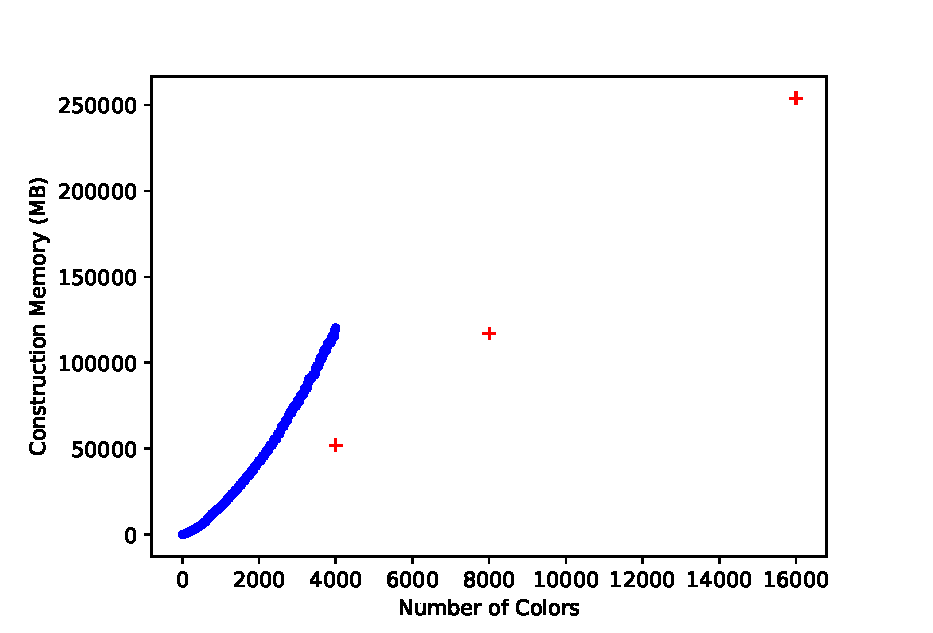
\includegraphics[scale=0.5]{content/BFTvsVARI.eps}
 %\caption{Comparison between Bloom Filter Trie (blue dots) and $\ours$ (red pluses) on isolates from GenomeTrakr.  Bloom Filter Trie was ran on 2,000 isolates and $\ours$ was ran on 4,000.}
 %\label{figure:bftvsvari}
%\end{figure*}


\begin{figure}[h!]
  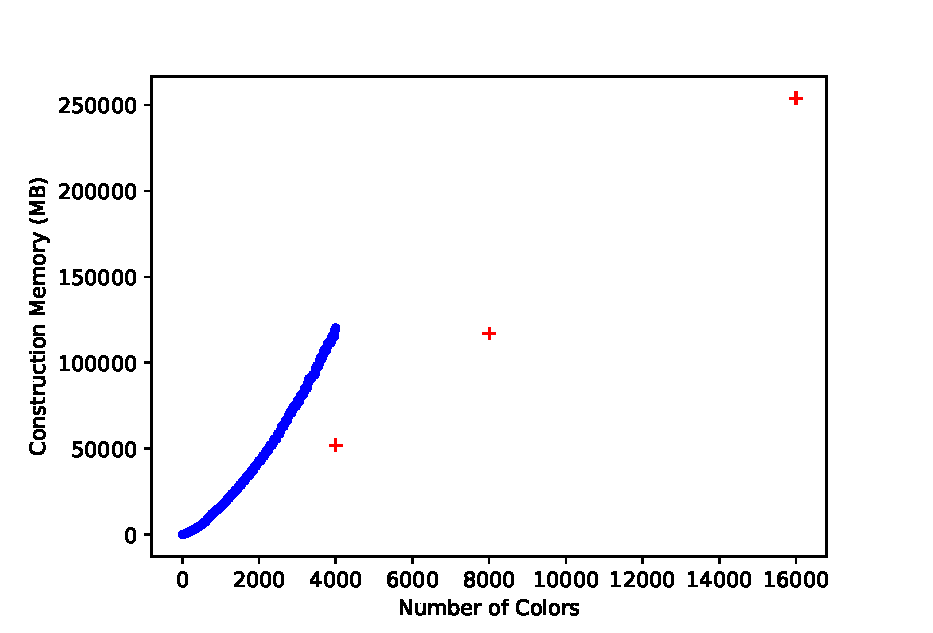
\includegraphics[width=0.55\textwidth]{content/BFTvsVARI.eps}
 \caption{Comparison between Bloom Filter Trie (blue dots) and $\ours$ (red pluses) on isolates from GenomeTrakr.  We ran Bloom Filter Trie on 4,000 isolates and plot $\ours$ results up through 16,000 isolates.}
 \label{figure:bftvsvari}
\end{figure}


\subsection{Comparison to Bloom Filter Trie}

In addition to demonstrating scalability, we used the Samonella strains from GenomeTrakr to directly compare the data structure space and construction memory of $\ours$ with Bloom Filter Trie~\cite{holley2015bloom} (BFT).  We observe both tools have a small memory overhead in construction above the final data structure. We found super-linear growth in BFT construction memory (see Figure \ref{figure:bftvsvari}), and that BFT produced a graph 105 GB in size after 4,000 samples were inserted. This is only slightly less space than the 106 GB the $\vari$ data structure requires to represent twice as many samples.  Holley  et al.~\cite{holley2015bloom} report  sub-linear growth up through 471 samples; however, we posit these differing observations may be a result of both differing dataset and preprocessing methods; More specifically, these isolates were extracted from a single species (humans) in contrast to GenomeTrakr, and thus may result in data that is more more homogeneous and has slower growth in the diversity with population size;  GenomeTrakr Salmonella samples are culled from  diverse food production environments.  Furthermore, they filter $k$-mers that have low multiplicity as a means to clean the data. This may reduce the growth as parts of the so called core genome may be missing in some samples, and the set of population $k$-mers could converge asymptotically toward the core genome.  Though Holley {\it et al.} compared to Sequence Bloom Trees by Solomon {\it et al.}~\cite{solomon2015large}, we do not because the Sequence Bloom Tree software is designed for transcript querying rather than variant detection.  %This may also contribute to different subsets of the true genomes content being considered by tools as datasets grow in size.

%We present Figure \ref{figure:bftvsvari} to illustrate the scalability of $\ours$ and Bloom Filter Trie.

%Preprocessing differences: They take raw reads, k-mer count them (k=63), and discard any k-mers with multiplicity less than 3.  This means k-mers covering read errors will likely be discarded, but might also leave chunks of the genome missing.  As more genomes are added, any 'core genome' components that are missing from individual sets could be found, so under this theory, one would expect the growth to be asymptotic toward capturing the whole 'core genome' in the data structure.  Perhaps this component dominates the growth giving the appearance of sublinear growth.  Under this theory, our assembly preprocessing could be keeping the bulk of the core genome and thus eliminate this component.  Other components of growth that were previously dominated might then become visible.

%Species/environment differences.  They are dealing with a different species and only those samples that can live in humans. So given the narrower environment there may be evolutionary pressure to select just the possible strains that thrive inside a human.  The salmonella in our dataset come from a much wider swath environments, so there is less selective pressure toward a more homogeneous population.  Thus the diversity of the underlying population itself grows faster which is then reflected in memory use.




% 4000 136gb ram, 1tb disk, 9 hours
% 8000 271gb ram, 4.6tb disk, 31hours


% 8000-merge 10gb ram, 6 hours

% 1. merge-2x2 vs vari-4, merge-4x4 vs vari8

% 2. vari, growth experiment with smaller things


% 3. incremental angle

% 4. bloom filter trie

% SO AND SO HAD 100 GENOMES AND ONLY BUILT THE DE BRUIJN GRAPH, but we were more efficient AND we included color too!


\subsection{Validation using E. coli}

%We copied the first $k$ nucleotides from the beginning of the FASTA sequence to the end in order to include $k$-mers lost when the circular genome is linearized to a disk file.

We validate $\ours$ by generating two succinct colored de Bruijn graphs with three \emph{E. coli} assemblies each, merge them, and verify correctness of the merged graph:    First, we generated all $k$-mers for each reference genome, counted all unique $k$-mers with KMC2~\cite{deorowicz2015kmc}, constructed two de Bruijn graphs of three assemblies each using $\vari$, and merged them into a six color graph using $\ours$.  Independently, we constructed a second colored de Bruijn graph using $\vari$ on all six assemblies in one run, and compared these two graphs.  We found $\ours$ produced files on disk that were bit-for-bit identical to those generated by $\vari$, demonstrating they construct equivalent graphs and data structures.

%Second, we partition each reference genome, leading to a de Bruin graph in which some nodes have no successors and others no predecessors.  We recall $\vari$ inserts extra edges for these conditions; however, some extra edges may become obsolete when graphs are merged.  In this situation, we expect the merged graph to have these additional obsolete extra edges relative to a graph built by $\vari$ from the complete set. We verify the equivalence of these graphs by printing the list of edges for the graph merged from two colored de Bruijn graphs (where the number of colors is equal to 3) as well as the colored de Bruijn graph (where the number of colors is equal to 6)  constructed using $\vari$.  We compared the full edge labels and found that the only difference was 126 additional extra edges in the merged graph.  Furthermore, applying VARI's bubble calling method to both graphs returned the same set of bubbles.


 

%\section{Discussion}
\section{Discussion and Conclusions} \label{sec:discussion} 

%To the best of our knowledge, t
This paper describes the first non-proprietary computational method for identifying misassembly errors using short read sequence data and optical mapping data.
% has not been previously considered using non-proprietary software.  
 Our results demonstrate: (1) a substantial number of misassembly errors can be identified in draft genomes of prokaryote and eukaryote speices; (2) our method scales to large genomes; and (3) it can be used in combination with any
 assembler and thus, making it a viable post-processing step for any assembly. 

While $\sequel$ is capable of identifying a significant percentage of misassembly errors, it does not address 
%the additional problem of re-assembling 
the reassembly of those the misassembled contigs. 
Correcting misassembly errors by segmenting the contigs at their breakpoints will remove the errors but will also 
%have the detrimental effect of reducing 
reduce
the N50 
of the assembly.  
For this reason, we believe that creating a reassembly tool to correctly reassemble contigs using the misassembly information and data warrants future investigation.
%Related to this problem is that of distinguishing between locally misassembled contigs and extensively misassembled contigs, which also deserves consideration.
%Hence, since SEQuel~\cite{sequel} is capable of correcting small indels and substitution errors, and $\sequel$ has the added virtue of identifying larger misassembly errors, the remaining step is to reassemble these contigs so that N50 is not degraded

While our main contributions are the computational method itself and the demonstration that optical mapping can have significant benefit for misassembly detection, optimal results are contingent upon good enzyme selection. 
Thus, we conclude by suggesting that efficient algorithmic selection of enzymes that will yield such informative optical maps in a {\em de novo} scenario is an area for interesting and important future work.  


%Moreover, the development of more sophisticated approaches to missassembly verification using optical mapping than just the presence or absence of alignments may further improve upon the results in this paper. Potential approaches include considering consistent estimated alignment loci in the genome across all optical maps, and determining the existence of unique, non-overlapping placement of each correctly assembled contig.

% We may want to add somewhere that some applications may prefer a method that favors good TPR vs FPR or vice versa and that while we've focused on a good balance, different alignment thresholds (or delta values for sequel) and combination strategies can shift this balance.






%%%%%%%%%%%%%%%%%%%%%%%%%%%%%%%%%%%%%%%%%%%%%%%%%%%%%%%%%%%%%%%%%%%%%%%%%%%%%%%%%%%%%
%
%     please remove the " % " symbol from \centerline{\includegraphics{fig01.eps}}
%     as it may ignore the figures.
%
%%%%%%%%%%%%%%%%%%%%%%%%%%%%%%%%%%%%%%%%%%%%%%%%%%%%%%%%%%%%%%%%%%%%%%%%%%%%%%%%%%%%%%






%\section{Conclusion}


\section*{Acknowledgement}
The authors would like to thank Journi Sir\'{e}n from the Wellcome Trust Sanger Institute for many insightful discussions, and Zamin Iqbal for his assistance with testing {\sc Cortex}.  

%\paragraph{Funding\textcolon} 

%\bibliographystyle{natbib}
%\bibliographystyle{achemnat}
%\bibliographystyle{plainnat}
%\bibliographystyle{abbrv}
%\bibliographystyle{bioinformatics}
%
%\bibliographystyle{plain}
%
%\bibliography{Document}



\bibliographystyle{natbib}
\bibliography{cdbg}


%% \begin{thebibliography}{}
%% \bibitem[Bofelli {\it et~al}., 2000]{Boffelli03} Bofelli,F., Name2, Name3 (2003) Article title, {\it Journal Name}, {\bf 199}, 133-154.

%% \bibitem[Bag {\it et~al}., 2001]{Bag01} Bag,M., Name2, Name3 (2001) Article title, {\it Journal Name}, {\bf 99}, 33-54.

%% \bibitem[Yoo \textit{et~al}., 2003]{Yoo03}
%% Yoo,M.S. \textit{et~al}. (2003) Oxidative stress regulated genes
%% in nigral dopaminergic neurnol cell: correlation with the known
%% pathology in Parkinson's disease. \textit{Brain Res. Mol. Brain
%% Res.}, \textbf{110}(Suppl. 1), 76--84.

%% \bibitem[Lehmann, 1986]{Leh86}
%% Lehmann,E.L. (1986) Chapter title. \textit{Book Title}. Vol.~1, 2nd edn. Springer-Verlag, New York.

%% \bibitem[Crenshaw and Jones, 2003]{Cre03}
%% Crenshaw, B.,III, and Jones, W.B.,Jr (2003) The future of clinical
%% cancer management: one tumor, one chip. \textit{Bioinformatics},
%% doi:10.1093/bioinformatics/btn000.

%% \bibitem[Auhtor \textit{et~al}. (2000)]{Aut00}
%% Auhtor,A.B. \textit{et~al}. (2000) Chapter title. In Smith, A.C.
%% (ed.), \textit{Book Title}, 2nd edn. Publisher, Location, Vol. 1, pp.
%% ???--???.

%% \bibitem[Bardet, 1920]{Bar20}
%% Bardet, G. (1920) Sur un syndrome d'obesite infantile avec
%% polydactylie et retinite pigmentaire (contribution a l'etude des
%% formes cliniques de l'obesite hypophysaire). PhD Thesis, name of
%% institution, Paris, France.

%% \end{thebibliography}
\end{document}
